\documentclass[../intro.tex]{subfiles}
\begin{document}

\section{Notation \& Definitions}

\begin{equation}
    A: \Gamma(E) \rightarrow \Gamma(H)
\end{equation}


 
\subsection{Data Space}
\begin{figure}[ht]
    \label{fig:mobius}
    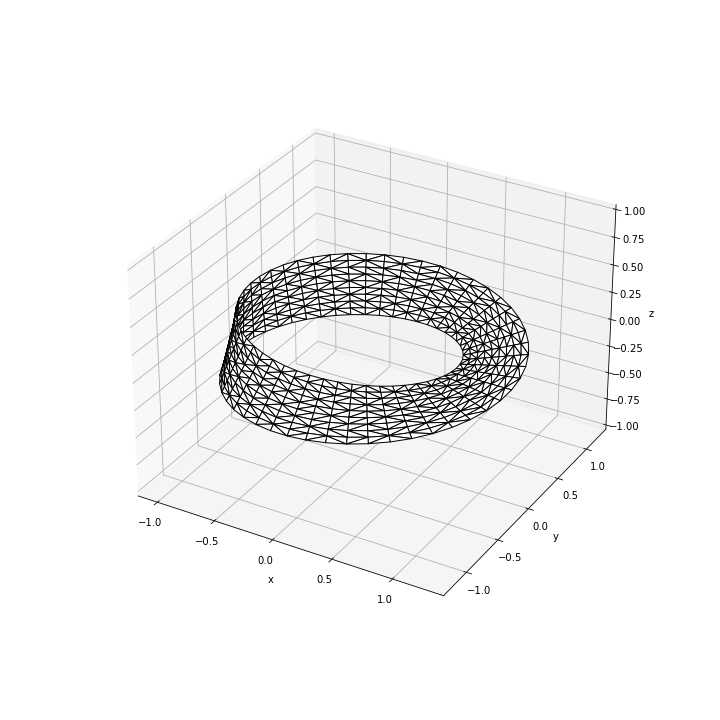
\includegraphics[width=0.5\linewidth]{figures/sections/math/mobius.png}
    \caption{write up some words here}
\end{figure}

We use a fiber bundle model to represent the data, as proposed by Butler 
\cite{butlerVectorBundleClassesForm1992,butlerVisualizationModelBased1989}. 


One example of a fiber bundle is the mobius band shown in figure~\ref{fig:mobius}. A fiber bundle is a topological total space $E$ with an embedded fiber space $F$, a base space on which the fibers lie $K$ and the $\pi$ and $\sigma$ mappings between $E$ and $K$.  

\begin{tikzcd}
    F \arrow[r, hook] & E \arrow[d, "\pi" description, bend right ] \\
                      & K \arrow[u, "\sigma" description, bend right]
\end{tikzcd}

As illustrated by the mobius band example in figure~\ref{fig:mobius}, the vertical lines $F$ are the range of possible values embedded in $E$ and the circle $K$ is a representation of the connectivity of the points in $E$. The function $\pi$ is the mapping from a point on a specific fiber $F_{k}|k\in K$ in $E$ to a location $k \in K$, and the section $\sigma$ is the mapping from a location $k$ on $K$ to a point on $F_{k}$ in $E$. The line $\Gamma$ is a space of sections


\subsubsection{Base Space $K$}

\begin{figure}[ht]
    \label{fig:simplex}
    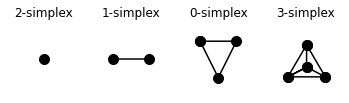
\includegraphics{figures/sections/math/simplex.png}
    \caption{Simplices encode the connectivity of the data, from fully disconnected (0 simplex) observations to all observations are connected to at least 3 other observations. Higher order simplicies are outside the scope of this paper.}
\end{figure}

One way to represent the topological space K is as a set composed of simplices, such as those shown in figure~\ref{fig:simplex}. Simplices are a way of encoding the connectivity of each observation ($\sigma(k)$) to another:

\begin{description}
    \item[0-simplex] discrete observations (inventory records)
    \item[1-simplex] 1D continuos data (timeseries)
    \item[2-simplex] 2D continuos data (map)
    \item[3-simplex] 3D continuos data (video)
\end{description}

In a locally trivial fiber bundle $E = F \times K$, it can be assumed that all $F_{k}$ for $k \in K$ are equal. A fiber bundle can be made locally trivial by approximating the total space E as a simplacial complex.

\subsubsection{Fiber Space $F$}
The fibers encode the set of all possible values each observation can take. 
Spivak's \cite{spivakSIMPLICIALDATABASES} formulation of the fibers as a union of named types gives a way to separate the values in the fiber by type:

\subsubsection{Subset \& Streaming}
$\Gamma(E)$ is the space of all points in $F$ returned by $\sigma$; therefore the points being visualized in a streaming or animation example can be considered a subset that lives on base space $U$ embedded in $K$ with the same fiber $\iota^*E$ and $\iota^*\sigma$.   

\begin{tikzcd}
    \iota^\ast E \arrow[r, hook] \arrow[d] & E \arrow[d]\\
    U \arrow[r, "\iota" description, hook] \arrow[u, "\iota^\ast \sigma" description, bend right,] & K \arrow[u, "\sigma" description, bend right]
\end{tikzcd}
%%% sheaves & presheaves 


\subsection{Visual Space}
%%render image
\begin{tikzcd}
    \mathbb{R}^{7} \arrow[r, hook] & H \arrow[d, "\zeta" description, bend right] \\
                                   & S \arrow[u, "\rho" description, bend right] 
\end{tikzcd}

%%% R7 in H, S base space, mostly will be trivial case H = S\times R^{7}

%% region on screen that corresponds to selection on H that corresponds to selection on S
The arrow in figure~\ref{fig:pullback} is an illustration of the lookup function $$f:\tau \rightarrow \mathbb{R}^7$$ returned by $$\mathbb{A}$$. The screen (represented by ~\ref{fig:pullback}(d)) queries the topological space $\mathbb{T}$ that underlies the ideal (realworld coordinate free) visual idiom (~\ref{fig:pullback}(c)) of the image. This idealized representations toplogy can be encoded as a 3 simplex since screens are ultimaltely 3 dimensional   

%%A: \Gamma(V) \rightarrow \Gamma(S)

%%f: \S \rightarrow R^{7} 

%%make bounding box bigger, pull in more rows (for averaging), bounding box on triangle, table is integral on bounding box - R,G,B, A = $$ \integral f(a,b)$$  (R, G, B, A functions )

draw functions return the renderer - T simplex 
set segments etc are currying f
(sampled, would be a table, visualizer can create different triangles/triangles based on renderer, invariances would hold - curremtly it's a png/r7 lookup table)

f to rnedring is lossy process
S - (face/collection of faces) <- simplicial complex, details encoded many ways dependent on renderer, connectivity is in line or edge (can also show multiple triangles...)

in practice w/ a renderer we have one triangle

(change f to rho)

\begin{equation}
    A: \Gamma(E) \rightarrow \Gamma(H)
\end{equation}

%%\psi map from S to topological K...
\subsubsection{Visual Idioms: Equivalance class of artists}
Visual Idioms

\subsubsection{Visual Variable Invariance}
Tau can preserves the measurement type properties (group scales)

Will implement in code such that this happens. 


\end{document}